\documentclass[11pt]{article}

% --- Packages (The "plugins" of LaTeX) ---
\usepackage[utf8]{inputenc} % Character encoding
\usepackage{geometry}       % Page margins
 \geometry{margin=1in}
\usepackage{graphicx}       % For inserting images
\usepackage{amsmath}        % For math equations
\usepackage{listings}
\usepackage{xcolor} % Required for syntax highlighting colors
\usepackage{booktabs} % For professional lines
\usepackage{siunitx}  % For decimal alignment

% Define colors for Python syntax
\definecolor{codegreen}{rgb}{0,0.6,0}
\definecolor{codegray}{rgb}{0.5,0.5,0.5}
\definecolor{codepurple}{rgb}{0.58,0,0.82}
\definecolor{backcolour}{rgb}{0.95,0.95,0.92}
\definecolor{termback}{rgb}{0.1,0.1,0.1}
\definecolor{termtext}{rgb}{0.9,0.9,0.9}
\definecolor{lightgray}{rgb}{0.9,0.9,0.9}

\lstdefinestyle{mystyle}{
    backgroundcolor=\color{backcolour},   
    commentstyle=\color{codegreen},
    keywordstyle=\color{magenta},
    numberstyle=\tiny\color{codegray},
    stringstyle=\color{codepurple},
    basicstyle=\ttfamily\footnotesize,
    breakatwhitespace=false,         
    breaklines=true,                 
    captionpos=b,                    
    keepspaces=true,                 
    numbers=left,                    
    numbersep=5pt,                  
    showspaces=false,                
    showstringspaces=false,
    showtabs=false,                  
    tabsize=2
}

\lstdefinestyle{terminal}{
    backgroundcolor=\color{white},   % White background
    basicstyle=\ttfamily\small\color{black}, % Black text
    frame=single,                    % Simple border
    rulecolor=\color{lightgray},     % Light gray border color
    breaklines=true,                 % Wrap long lines
    numbers=none,                    % No line numbers for output
    captionpos=b,                    % Caption at the bottom
    xleftmargin=10pt,                
    xrightmargin=10pt,
    framesep=5pt
}

\lstset{style=mystyle}

% --- Document Information ---
\title{DE 414: Practical 5 Report}
\author{Amy McDermott (26911264)}
\date{\today}

\begin{document}

\maketitle

\section*{Introduction}
This report documents the implementation of a Convolutional Neural Network using PyTorch. It explores defining the CNN model structure, training the model, 
and visualising trained CNN filters. The CNN is designed to classify images from the MNIST dataset.

\section*{Question 1: Loading the data}
The function \texttt{load\_npz} is used to load the MNIST dataset from a .npz file. The dataset is split into training and test sets, and the shapes of the loaded data are printed to confirm successful loading.
The loaded data consists of 60000 training samples and 10000 test samples, with each image flattened into a 784-dimensional vector (28x28 pixels), as shown in the terminal output in Listing \ref{lst:loadingdata}.
\begin{lstlisting}[
    language=Python, 
    caption={Terminal output showing the dimensions of the loaded MNIST dataset.},
    label={lst:loadingdata},
    breaklines=true,
    basicstyle=\ttfamily\small,
    frame=single
]
+----------------------------------------
| Train X: torch.Size([60000, 784])
| Train Y: torch.Siz1: Defining the CNN Modele([60000])
| Test X: torch.Size([10000, 784])
| Test Y: torch.Size([10000])
+ ----------------------------------------
\end{lstlisting}

\section*{Question 2}
\subsection*{Question 2.1: Defining the CNN model structure}
The CNN is defined using PyTorch's \texttt{nn.Module} class, and the layers are initialised in the constuctor. The CNN layer takes the input image and applies convolution to extract features, 
while the ReLU activation function introduces non-linearity so that the network can learn complex patterns. The fully connected layer takes the flattened output from the CNN layer and produces the final class scores for classification.
The model parameters are set to ensure that the output dimensions of each layer are compatible, allowing the data to flow correctly through the network. The CNN layer outputs a matrix of size 11x11 with 10 channels, which is then flattened to a vector of size 1210 before being passed to the dense layer for classification into 10 classes (digits 0-9). 
\begin{itemize}
    \item CNN layer: P1 = P2 = 28, P3 = 1, M1 = M2 = 8, M3 = 10, S = 2
    \item ReLU activation: Q1 = Q2 = 11, Q3 = 10
    \item Dense layer: P = 1210, Q = 10
\end{itemize}
The code snippet in Listing \ref{lst:cnnmodel} shows the definition of the CNN model structure in PyTorch.

\begin{lstlisting}[
    language=Python, 
    caption={Definition of the CNN model structure.},
    label={lst:cnnmodel},
    breaklines=true,
    basicstyle=\ttfamily\small,
    frame=single
]
self.conv_1 = nn.Conv2d(in_channels=1, out_channels=M_3, kernel_size=(M_1,M_2), stride=stride)
self.relu = nn.ReLU()
# Input to the linear layer is the flattened version of the conv output (i.e. 11 x 11 x 10 = 1210) and output is K = 10
self.linear = nn.Linear(in_features=1210, out_features=K)
\end{lstlisting}

\subsection*{Question 2.2: Implementing the forward pass}
The forward pass is then implemented to define how the input data flows through the network layers. The input image is reshaped to match the expected 
input dimensions of the CNN layer, and the output from the convolutional layer is passed through the ReLU activation function before being flattened and fed into the dense layer for classification.
\begin{lstlisting}[
    language=Python, 
    caption={Implementation of the forward pass through the CNN model.},
    label={lst:forwardpass},
    breaklines=true,
    basicstyle=\ttfamily\small,
    frame=single
]
# Convolutional layers expect input in the format (Batch size, Channels, Height, Width)
z_1 = self.conv_1(x.view(-1,1,28,28)) # reshape input to (N,1,28,28) for CNN layer
v_1 = self.relu(z_1)
# flatten the output of the convolutional layer (i.e. 11 x 11 x 10 = 1210)
v_1_flat = torch.flatten(v_1,start_dim=1) # flatten before passing to the dense layer
y_hat = self.linear(v_1_flat)
\end{lstlisting}

\subsection*{Question 2.3: Instantiating the model}
The model is instantiated by creating an instance of the CNN class defined in Question 2. Cross entropy loss function as well as an SGD optimiser is then defined. 
Model parameters are defined: learning rate = 0.01, batch size = 30 and epochs = 10. The model summary is printed out to confirm the architecture and the number of parameters in each layer, as shown in the terminal output in Listing \ref{lst:modelsummary}.

\begin{lstlisting}[
    language=Python, 
    caption={Instantiating the CNN model and defining the loss function and optimizer.},
    label={lst:instantiatingmodel},
    breaklines=true,
    basicstyle=\ttfamily\small,
    frame=single
]
model = CNN(8,8,10,10,2) # define model
loss_fn = nn.CrossEntropyLoss() # define loss function
optimizer = torch.optim.SGD(model.parameters(), lr=lr) # define optimizer
\end{lstlisting}

\begin{lstlisting}[
    language=Python, 
    caption={Terminal output showing the model summary.},
    label={lst:modelsummary},
    breaklines=true,
    basicstyle=\ttfamily\small,
    frame=single
]
CNN(
  (conv_1): Conv2d(1, 10, kernel_size=(8, 8), stride=(2, 2))
  (relu): ReLU()
  (linear): Linear(in_features=1210, out_features=10, bias=True)
)
\end{lstlisting}

\subsection*{Question 3: Training the model}

The model was trained over a number of epochs, where in each epoch the training data was iterated through in batches. 
For each batch, a forward pass was performed to calculate the model's predictions, and the loss was determined using these predictions and the target labels. 
Then, the gradients were calculated using a backward pass, and the model's parameters were updated using the optimizer.
The training loss as well as the training accuracy (i.e. percentage of examples in the batch that were correctly classified) are tracked and printed out at the end of each epoch.
Note that the model was set to training mode during the training loop.
\begin{lstlisting}[
    language=Python, 
    caption={Model training loop, showing the process of forward pass, loss calculation, backward pass, and parameter updates.},
    label={lst:modeltraining},
    breaklines=true,
    basicstyle=\ttfamily\small,
    frame=single
]
y_hat = model(X_i)[0] # forward pass - model prediction
loss = loss_fn(y_hat, y_i) # calculate training loss

# clear gradients on all optimised tensors, otherwise gradients accumulate on subsequent backward passes
optimizer.zero_grad() 
loss.backward() # calculate gradients
optimizer.step() # update model parameters using the calculated gradients
\end{lstlisting}   

The model is also evaluated on the test set at the end of each epoch to track the test loss and test accuracy. The model is set 
to evaluation mode, and the forward pass and loss calculation then proceed to take place.
The test loss and test accuracy are computed for each epoch and printed out alongside the training loss and training accuracy, as shown in the terminal output in Listing \ref{lst:trainingperformance}.
Mention a point here on model test accuracy - starts to overfit?
Listing \ref{lst:modeltesting} shows the code snippet for evaluating the model on the test set throughout the model training process.
\begin{lstlisting}[
    language=Python, 
    caption={Model evaluation on the test set during training, showing the forward pass and loss calculation for the test data.},
    label={lst:modeltesting},
    breaklines=true,
    basicstyle=\ttfamily\small,
    frame=single
]
y_hat = model(X_i)[0]
loss = loss_fn(y_hat, y_i)
# track the test loss and accuracy
test_loss += loss.item() * test_batch_size
test_accuracy += hits(y_hat,y_i)
\end{lstlisting}  

\begin{lstlisting}[
    language=Python, 
    caption={Model epoch performance during training, showing loss and accuracy for both training and test sets.},
    label={lst:trainingperformance},
    breaklines=true,
    basicstyle=\ttfamily\small,
    frame=single
]
****************************************
Beginning training
Epoch 1 Loss: 0.0740 Accuracy: 97.90 Test Loss: 0.0735 Test Accuracy: 97.84
Epoch 2 Loss: 0.0701 Accuracy: 98.00 Test Loss: 0.0705 Test Accuracy: 97.97
Epoch 3 Loss: 0.0668 Accuracy: 98.11 Test Loss: 0.0679 Test Accuracy: 98.02
Epoch 4 Loss: 0.0639 Accuracy: 98.19 Test Loss: 0.0657 Test Accuracy: 98.07
Epoch 5 Loss: 0.0614 Accuracy: 98.26 Test Loss: 0.0637 Test Accuracy: 98.07
Epoch 6 Loss: 0.0591 Accuracy: 98.32 Test Loss: 0.0620 Test Accuracy: 98.09
Epoch 7 Loss: 0.0570 Accuracy: 98.37 Test Loss: 0.0605 Test Accuracy: 98.14
Epoch 8 Loss: 0.0552 Accuracy: 98.42 Test Loss: 0.0592 Test Accuracy: 98.19
Epoch 9 Loss: 0.0535 Accuracy: 98.47 Test Loss: 0.0580 Test Accuracy: 98.18
Epoch 10 Loss: 0.0519 Accuracy: 98.53 Test Loss: 0.0570 Test Accuracy: 98.18
\end{lstlisting}

\subsection*{Question 4: Visualising trained CNN filters}
An instance of data from the test set is fed through the model and its corresponding filters and correlations are plotted using the \texttt{plot\_filters} function. 
This is executed by initially extracting the first sample from the test set, then extracting the weights from the convolutional layer of the model, and finally performing
a forward pass for the sample from the test set to obtain the network outputs y\_hat, z\_1 and v\_1. The \texttt{plot\_filters} function is then called with the appropriate arguments to visualise the filters and correlations. 
The resulting visualisation of the trained CNN filters is shown in Figure \ref{fig:trainingfilters}. 

\begin{lstlisting}[
    language=Python, 
    caption={Visualisation of the trained CNN filters.},
    label={lst:visualisefilters},
    breaklines=true,
    basicstyle=\ttfamily\small,
    frame=single
]
X = test_X[0:1, :] # sample to be fed to your model 
H = model.conv_1.weight.detach() # extract the weights from the convolutional layer and detach from computational graph
model.eval() # set model to evaluation mode
with torch.no_grad(): # stop tracking gradients for the forward pass
  y_hat, z_1, v_1 = model(X) # forward pass for the sample

plot_filters(X.detach(), H, z_1.detach(), v_1.detach()) # plot the filters and correlations
\end{lstlisting}  

\begin{figure}[htbp]
    \centering
    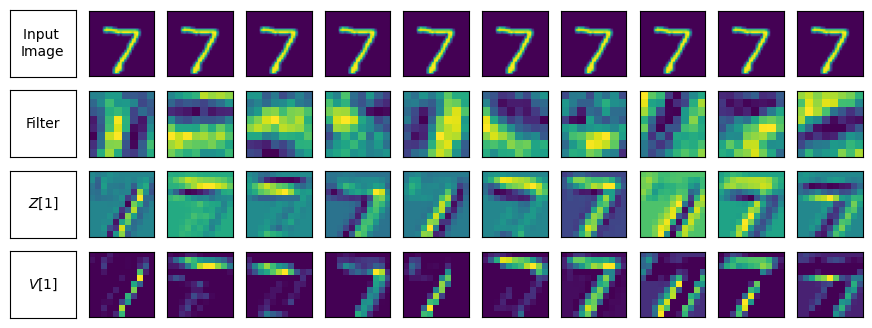
\includegraphics[width=0.85\linewidth]{Q4.png}
    \caption{Visualisation of the trained CNN filters.}
    \label{fig:trainingfilters}
\end{figure}



\end{document}